%HW10.tex
%Tenth Homework -- Math 221H
% 
%
% Frank Sottile
% 29 October 2023 
%
%%%%%%%%%%%%%%%%%%%%%%%%%%%%%%%%%%%%%%%%%%%%%%%%%%%%%%%%
\documentclass[12pt]{article}
\usepackage{amssymb,amsmath}
\usepackage{graphicx}
\usepackage[usenames,dvipsnames,svgnames,table]{xcolor}
\usepackage{multirow}   % This is for more control over tables
%%%%%%%%%%%%%%%%%%%%%%%%%%%%%%%%  Layout     %%%%%%%%%%%%%%%%%%%%%%%%%%%%%%%%%%%%%%
\usepackage{vmargin}
\setpapersize{USletter}
\setmargrb{1cm}{0.25cm}{1cm}{0.5cm} % --- sets all four margins LTRB

%%%%%%%%%%%%%%%%%%%%%%%%%%%%%%%%%%%%%%%%  Macros  %%%%%%%%%%%%%%%%%%%%%%%%%%%%%%%%%%%%%%%%
\newcommand{\RR}{{\mathbb R}}  % This is the backboard bold symbol for the real numbers.  Note how it is used below
\newcommand{\NN}{{\mathbb N}}  % 
\newcommand{\ZZ}{{\mathbb Z}}  %

\newcommand{\calP}{{\mathcal P}}  %Caligraphic P for power set

\newcommand{\bfa}{{\bf a}}    %Vectors
\newcommand{\bfb}{{\bf b}}    %Vectors
\newcommand{\bfi}{{\bf i}}    %Unit Vectors
\newcommand{\bfj}{{\bf j}}    %Unit Vectors
\newcommand{\bfk}{{\bf k}}    %Unit Vectors

\newcommand{\sep}{{\ :\ }}     % This is for the : in our notation for building sets.
                               % an acceptable (and common) alternative is \mid  (try it!)
%%%%%%%%%%%%%%%%%%%%%%%%%%%%%%%%%%%%%%%%%%%%%%%%%%%%%%%%%%%%%%%%%%%%%%%%
\begin{document}
\LARGE 
\noindent
{\color{Maroon}Honors Multivariate Calculus \hfill Math 221H Section 201}\vspace{2pt}\\
\large
Tenth Homework:\hfill 
Due in recitation: Thursday 2 November 2023\vspace{2pt}

\normalsize
    \vspace{2pt}

%%%%%%%%%%%%%%%%%%%%%%%%%%%%%%%%%%%%%%%%%%%%%%%%%%%%%%%%%%%%%%%%%%%%%%%%%%%%%%%%%%%%%%%%%%%%%%%%%%%%
\begin{enumerate}



%%%%%%%%%%%%%%%%%%%%%%%%%%%%%%%%%%%%%%%%%%%%%%%%%%%%%%%%%%%%%%%%%%%%%%%%%%%%%%%%%%%%%%%%%%%%%%%%%%%%
\item Evaluate the following improper integrals.

  (a) ${\displaystyle \int_{-\infty}^\infty x^2 e^{-x^2}\, dx}$
  \qquad and \qquad
  (b) ${\displaystyle \int_{-\infty}^\infty \sqrt{x} e^{-x}\, dx}$\,.
  
\vspace{-2pt}
%%%%%%%%%%%%%%%%%%%%%%%%%%%%%%%%%%%%%%%%%%%%%%%%%%%%%%%%%%%%%%%%%%%%%%%%%%%%%%%%%%%%%%%%%%%%%%%%%%%%
   
%%%%%%%%%%%%%%%%%%%%%%%%%%%%%%%%%%%%%%%%%%%%%%%%%%%%%%%%%%%%%%%%%%%%%%%%%%%%%%%%%%%%%%%%%%%%%%%%%%%%
\item Electric charge is distributed over the disk $x^2+y^2\leq 2$ with charge density $\sigma(x,y)=1+x^2+y^2$.
  Find the total charge on the disk.
\vspace{-2pt}
%%%%%%%%%%%%%%%%%%%%%%%%%%%%%%%%%%%%%%%%%%%%%%%%%%%%%%%%%%%%%%%%%%%%%%%%%%%%%%%%%%%%%%%%%%%%%%%%%%%%
   


%%%%%%%%%%%%%%%%%%%%%%%%%%%%%%%%%%%%%%%%%%%%%%%%%%%%%%%%%%%%%%%%%%%%%%%%%%%%%%%%%%%%%%%%%%%%%%%%%%%%
\item A lamina (thin sheet of material) occupies the region inside the circle $x^2+y^2=2y$ but outside the unit circle
  $x^2+y^2=1$.
  Find its center of mass if the density at any point is inversely proportional to its distance to the origin.
\vspace{-2pt}
%%%%%%%%%%%%%%%%%%%%%%%%%%%%%%%%%%%%%%%%%%%%%%%%%%%%%%%%%%%%%%%%%%%%%%%%%%%%%%%%%%%%%%%%%%%%%%%%%%%%
   



%%%%%%%%%%%%%%%%%%%%%%%%%%%%%%%%%%%%%%%%%%%%%%%%%%%%%%%%%%%%%%%%%%%%%%%%%%%%%%%%%%%%%%%%%%%%%%%%%%%%
\item A lamina  has shape that part of the disk $x^2+y^2\leq 4$ that lies in the first quadrant.
  Suppose that its mass density is proportional to the square of the distance to the origin, $\rho(x,y)=k(x^2+y^2)$.
  Find its center of mass.
\vspace{-2pt}
%%%%%%%%%%%%%%%%%%%%%%%%%%%%%%%%%%%%%%%%%%%%%%%%%%%%%%%%%%%%%%%%%%%%%%%%%%%%%%%%%%%%%%%%%%%%%%%%%%%%
   

%%%%%%%%%%%%%%%%%%%%%%%%%%%%%%%%%%%%%%%%%%%%%%%%%%%%%%%%%%%%%%%%%%%%%%%%%%%%%%%%%%%%%%%%%%%%%%%%%%%%
\item Suppose that a lamina is in the shape of the rectangle $D=\{(x,y)\mid 0\leq x\leq 2\,,\ 0\leq y\leq 3\}$ with mass density
  $\rho(x,y)=\pi y$.
  Find its center of mass.
\vspace{-2pt}
%%%%%%%%%%%%%%%%%%%%%%%%%%%%%%%%%%%%%%%%%%%%%%%%%%%%%%%%%%%%%%%%%%%%%%%%%%%%%%%%%%%%%%%%%%%%%%%%%%%%
   

%%%%%%%%%%%%%%%%%%%%%%%%%%%%%%%%%%%%%%%%%%%%%%%%%%%%%%%%%%%%%%%%%%%%%%%%%%%%%%%%%%%%%%%%%%%%%%%%%%%%
\item Find the three moments of inertial $I_x$, $I_y$, and $I_0$ \newline of the lamina from each of the previous two problems. 
\vspace{-2pt}
%%%%%%%%%%%%%%%%%%%%%%%%%%%%%%%%%%%%%%%%%%%%%%%%%%%%%%%%%%%%%%%%%%%%%%%%%%%%%%%%%%%%%%%%%%%%%%%%%%%%
   


%%%%%%%%%%%%%%%%%%%%%%%%%%%%%%%%%%%%%%%%%%%%%%%%%%%%%%%%%%%%%%%%%%%%%%%%%%%%%%%%  
 \item   
  \begin{minipage}[t]{3.8in}
    Suppose that a lamina is in the shape of the cardiod  $r=2-2\sin(\theta)$ with constant mass density.
    Find its centroid and three moments of inertial $I_x$, $I_y$, and $I_0$.
  \end{minipage}
  \begin{minipage}[t]{110pt}
   \raisebox{-10pt}{
\begin{picture}(105,5)(-10,30)
 \put(0,0){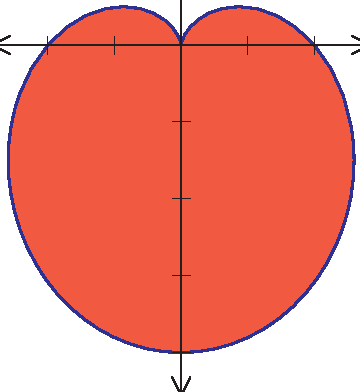
\includegraphics[height=95pt]{images/HW10_1}}
\end{picture}}
  \end{minipage}
%%%%%%%%%%%%%%%%%%%%%%%%%%%%%%%%%%%%%%%%%%%%%%%%%%%%%%%%%%%%%%%%%%%%%%%%%%%%%%%%  


%%%%%%%%%%%%%%%%%%%%%%%%%%%%%%%%%%%%%%%%%%%%%%%%%%%%%%%%%%%%%%%%%%%%%%%%%%%%%%%%%%%%%%%%%%%%%%%%%%%%
\item
  \begin{minipage}[t]{5.2in}
    Repeat the previous exercise, but for the first loop \newline
    (in the positive quadrant) of the four-leaved rose  \newline $r=2\sin(2\theta)$.
    (Use symmetry to
    reduce your workload.)
  \end{minipage}
  \begin{minipage}[t]{60pt}
   \begin{picture}(65,5)(-20,70)
    \put(0,0){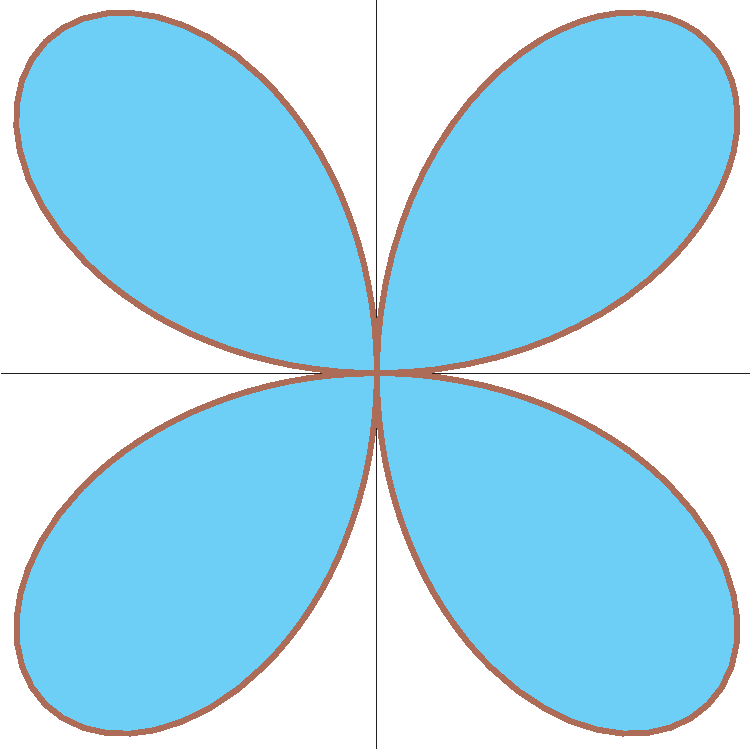
\includegraphics[height=120pt]{images/HW10_2}}
    \end{picture}
  \end{minipage}
\vspace{-2pt}
%%%%%%%%%%%%%%%%%%%%%%%%%%%%%%%%%%%%%%%%%%%%%%%%%%%%%%%%%%%%%%%%%%%%%%%%%%%%%%%%%%%%%%%%%%%%%%%%%%%%
   

%%%%%%%%%%%%%%%%%%%%%%%%%%%%%%%%%%%%%%%%%%%%%%%%%%%%%%%%%%%%%%%%%%%%%%%%%%%%%%%%%%%%%%%%%%%%%%%%%%%%
\item Repeat the previous exercise, but for the full area enclosed by the \newline four-leaved rose $r=2\sin(2\theta)$.
  (Again, use symmetry.)
\vspace{-2pt}
%%%%%%%%%%%%%%%%%%%%%%%%%%%%%%%%%%%%%%%%%%%%%%%%%%%%%%%%%%%%%%%%%%%%%%%%%%%%%%%%%%%%%%%%%%%%%%%%%%%%
   


%%%%%%%%%%%%%%%%%%%%%%%%%%%%%%%%%%%%%%%%%%%%%%%%%%%%%%%%%%%%%%%%%%%%%%%%%%%%%%%%%%%%%%%%%%%%%%%%%%%%
\item Evaluate the iterated integral ${\displaystyle \int_0^3 \int_0^{\sqrt{9-x^2}} \int_0^x yz\, dy\, dz\, dx}$.
\vspace{-2pt}
%%%%%%%%%%%%%%%%%%%%%%%%%%%%%%%%%%%%%%%%%%%%%%%%%%%%%%%%%%%%%%%%%%%%%%%%%%%%%%%%%%%%%%%%%%%%%%%%%%%%
   

%%%%%%%%%%%%%%%%%%%%%%%%%%%%%%%%%%%%%%%%%%%%%%%%%%%%%%%%%%%%%%%%%%%%%%%%%%%%%%%%%%%%%%%%%%%%%%%%%%%%
\item Compute $\iiint_E xy\, dV$ where $E$ is the tetrahedron with vertices $(0,0,0)$, $(3,0,0)$, $(0,2,0)$, $(0,0,1)$.
\vspace{-2pt}
%%%%%%%%%%%%%%%%%%%%%%%%%%%%%%%%%%%%%%%%%%%%%%%%%%%%%%%%%%%%%%%%%%%%%%%%%%%%%%%%%%%%%%%%%%%%%%%%%%%%
  

%%%%%%%%%%%%%%%%%%%%%%%%%%%%%%%%%%%%%%%%%%%%%%%%%%%%%%%%%%%%%%%%%%%%%%%%%%%%%%%%%%%%%%%%%%%%%%%%%%%%
\item Compute $\iiint_E xy\, dV$ where $E$ is the solid bounded by the \newline
  parabolic cylinder $y=x^2$ and the planes $x=z$, $x=y$, and $z=0$.
\vspace{-2pt}
%%%%%%%%%%%%%%%%%%%%%%%%%%%%%%%%%%%%%%%%%%%%%%%%%%%%%%%%%%%%%%%%%%%%%%%%%%%%%%%%%%%%%%%%%%%%%%%%%%%%
 

%%%%%%%%%%%%%%%%%%%%%%%%%%%%%%%%%%%%%%%%%%%%%%%%%%%%%%%%%%%%%%%%%%%%%%%%%%%%%%%%%%%%%%%%%%%%%%%%%%%%
\item Express $\iiint_E f(x,y,z)\, dV$ as an iterated integral in six different \newline
  ways, where $E$ is the solid bounded by 
  $z=0$, $x=0$, $y=2$, and $z=y-2x$.
\vspace{-2pt}
%%%%%%%%%%%%%%%%%%%%%%%%%%%%%%%%%%%%%%%%%%%%%%%%%%%%%%%%%%%%%%%%%%%%%%%%%%%%%%%%%%%%%%%%%%%%%%%%%%%%
     

%%%%%%%%%%%%%%%%%%%%%%%%%%%%%%%%%%%%%%%%%%%%%%%%%%%%%%%%%%%%%%%%%%%%%%%%%%%%%%%%%%%%%%%%%%%%%%%%%%%%
\item
  \begin{minipage}[t]{5.2in}
    The figure shows the region of integration for the integral
    \[
    \int_0^1 \, \int_0^{1-x^2}\, \int_0^{1-x} f(x,y,z)\,dy\,dz\,dx\,.
    \]
    Rewrite this as an equivalent interated integral in the five other ways.
  \end{minipage}
  \begin{minipage}[t]{60pt}
   \begin{picture}(65,5)(0,60)
     \put(0,0){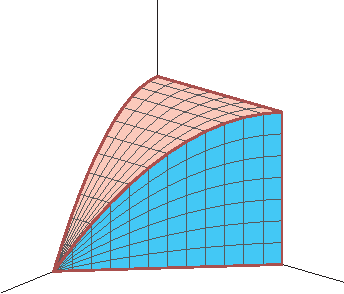
\includegraphics[height=130pt]{images/HW10_3}}

     \put( 0,6){\small$x$}    \put(71,123){\small$z$}     \put(145,11){\small$y$}
     \put(22,0){\small$1$}    \put(71, 98){\small$1$}     \put(122,3){\small$1$}

      \thicklines
         \put(55, -5){{\color{white}\vector(2,3){31}}}
         \put(55, -5.6){{\color{white}\line(2,3){30}}}
         \put(55, -5.3){{\color{white}\line(2,3){30}}}
         \put(55, -4.7){{\color{white}\line(2,3){30}}}
         \put(55, -4.4){{\color{white}\line(2,3){30}}}

          \put(30,100){{\color{white}\vector(1,-2){22}}}
          \put(30.6,100){{\color{white}\line(1,-2){21}}}
          \put(30.3,100){{\color{white}\line(1,-2){21}}}
          \put(29.7,100){{\color{white}\line(1,-2){21}}}
          \put(29.4,100){{\color{white}\line(1,-2){21}}}
    \thinlines
     
     \put(40,-15){\small$y=1-x$}    \put(55, -5){\vector(2,3){30}}
     \put( 0,105){\small$z=1-x^2$}  \put(30,100){\vector(1,-2){21}}
     
    \end{picture}
  \end{minipage}

%%%%%%%%%%%%%%%%%%%%%%%%%%%%%%%%%%%%%%%%%%%%%%%%%%%%%%%%%%%%%%%%%%%%%%%%%%%%%%%%%%%%%%%%%%%%%%%%%%%%
     


\end{enumerate}



\end{document}
%%%%%%%%%%%%%%%%%%%%%%%%%%%%%%%%%%%%%%%%%%%%%%%%%%%%%%%%%%%%%%%%%%%
polar/Lune
